\chapter{A Secure RDF Data Integration Framework}
\label{cha:usecase}

In this chapter we go back to the \usecase presented in \cref{cha:introduction}, where we briefly mentioned the several
software applications that enterprises use to manage their business: interactions with clients in a Customer
Relationship Management (CRM) application, employee information in a Human Resources (HR) application, project
documentation and company policies in a Document Management System (DMS) and records of time spent working on projects
in a Timesheet System (TS).
%
Heterogeneity of the data formats from the different software applications is not the only problem. In fact, as much of
the information within the enterprise is highly sensitive, its integration could result in information leakage to
unauthorised individuals.

In this chapter we build on the languages presented in the previous chapters to automatically extract data and access
control information from the underlying databases and represent them as Annotated \ac{RDF} graphs, providing a holistic
view of data across the enterprise. 
%
This approach introduces a mechanism to enforce access control policies on the \ac{RDF} graph along with a flexible and
automatic way to represent and propagate the original access control policies.

In this chapter we define an annotation domain that models access control permissions as Annotated RDFS, specify the
high-level system architecture required to enforce access control by relying on SPARQL, and illustrate how domain
specific rules can be used to manage the access control annotations.
%
First we present some common access control related terms that we use in this chapter:
%
\begin{description}[noitemsep]
\item[Resources] denote the information to be protected;
  % 
\item[Users] represent individuals requesting access to resources;
  % 
\item[Groups] are collections of users with common features (\eg~contributors, supervisors, and management);
  % 
\item[Roles] are commonly used to assign access rights to a set of individuals and groups, for example by department
  (\eg~human resources, sales and marketing) or task (\eg~insurance claim processing, reporting and invoicing).
  % 
\end{description}

\section{The Access Control Annotation Domain}
\label{sec:access-contr-doma}

In this section we formalise our access control annotation domain, following the definitions presented in
\cref{sec:rdfs-annot-doma}.  We start by defining the entities and annotation values and then present the~$\otimes$
and~$\oplus$ domain operations. Finally, we briefly describe the implementation of the presented annotation domain.


\subsection{Entities and Annotations}
\label{sec:modell-access-contr}


For the modelling of the access control domain consider, in addition to the previously presented sets of URIs \AU, blank
nodes \AB, and literals \AL, a set of credential elements~\AC.
%
The elements of~\AC are used to represent \emph{users}, \emph{roles}, and \emph{groups}.
%
To cater for \emph{attribute based access control}, we consider a set~\AT of pairs of form $k=v$, to be considered as
attribute-value pairs, where $k,v \in \AL$.  For example ``$age=30$'' or ``$institute=DERI$'' are elements
of~$\aset{T}$.  We allow shortcuts to represent intervals of integers, for example ``$age=[25,30]$'' to indicate that
all entities with attribute~$age$ between~$25$ and~$30$ are allowed access to the triple.

Considering an element $e \in \ACT$, $e$ and $\neg e$ are \emph{access control elements}, where~$e$ is called a
\emph{positive} element and~$\neg e$ is called a \emph{negative} element.\footnote{Here we are using $\neg e$ to
  represent strong negation.  In our access control domain representation, $\neg e$ indicates that $e$ will be
  specifically \emph{denied} access.}
%
An \emph{access control statement}~$S$ consists of a set of access control elements and we further consider that~$S$ is
in \emph{consistent} iff for any element~$e \in \ACT$, only one among $e$ and~$\neg e$ may appear in~$S$.  This
restriction avoids \emph{conflicts}, where a statement is attempting to both \emph{grant} and \emph{deny} access to a
triple.
%
Furthermore, we can define a partial order between statements as~$S_{1} \leq S_{2} \mbox{ iff\ } S_{1} \subseteq S_{2}$
that can be used to eliminate \emph{redundant} access permissions: if a user is granted access by statement~$S_{2}$, he
will also be granted access by statement~$S_{1}$ (and thus $S_{2}$ can be removed). 
%
Finally, an \emph{\ac{ACL}} consists of a set of access control statements and an \ac{ACL} is considered
\emph{consistent} iff each statement it contains is consistent and not redundant.  In our domain representation, only
consistent \acp{ACL} are considered as annotation values.
%
Intuitively, an annotation value specifies which entities have read permission to the triple, or are denied access when
the annotation is preceded by~$\neg$.
%
\begin{example}[Access Control List]
  %
  \label{ex:ann-value}
  We are considering the following set of entities~$\AC = \{ jb,js,st,it \}$, where $jb$ and $js$ are employee usernames
  and~$st$ and~$it$ are shorthand for~$\mathit{softwareTester}$ and~$\mathit{informationTechnology}$, respectively.
  % 
  The following annotated triple:
  $$\fuzzyg{\tau}{[[it],[st, \neg js]]}$$
  % 
  states that the entities identified with $it$ or $st$ (except if the $js$ credential is also present) have read access
  to the triple $\tau$.
\end{example}
%
An \ac{ACL}~$A$ can be considered as a non-recursive Datalog with negation (\nrdn) program, where access control
statement~$s \in A$ corresponds to the body of a rule in the Datalog program.
%
The head of the Datalog rules is a reserved literal $access \not\in\ACT$ and the evaluation of the Datalog program
determines the access permission to a triple for a specific set of credentials.

The set of user credentials is assumed to be provided by an external authentication service and consists of elements
of~\ACT, which equate to a non-empty \ac{ACL} representing the entities associated with the user.  We further assume
that this \ac{ACL} consists of only one positive statement, \ie~the \ac{ACL} will contain only one statement with all
the entities associated with the user and does not contain any negative elements.
%
\vspace{-10pt}
%
\begin{example}[Datalog Representation of an ACL]
  %
  \label{ex:datalog-program}
  Consider the annotation example presented in \cref{ex:ann-value}. The \nrdn program corresponding to the
  \ac{ACL}~$[[it],[st, \neg js]]$ is:
  %
  \begin{align*}
    access \leftarrow &~it .\\
    access \leftarrow &~st, \neg js .  
  \end{align*}
  % 
  The set of credentials of the user \emph{session}, provided by the external authentication system eg.~$[[jb,it]]$, are
  considered the facts in the \nrdn program.
\end{example}
%
Further domain specific information, for example hierarchies between the access control entities, can be encoded as
extra rules within the \nrdn program.  These extra rules can be used to provide \emph{implicit} credentials to a user,
allowing the access control to be specified based on credentials that the authentication system does not necessarily
assign to a user.
%
\begin{example}[Credential Hierarchies]
  Considering that the entity~$emp$ represents all the employees within a specific company, and that~$jb$ and~$js$
  correspond to employee usernames (as presented in \cref{ex:ann-value}), the following rules can be added to the
  \nrdn program from \cref{ex:datalog-program}:
  %
  \begin{align*}
    emp \leftarrow &~ js .\\
    emp \leftarrow &~ jb .  
  \end{align*}
  % 
  These rules ensure that both~$jb$ and~$js$ are given access when the credential~$emp$ is required in an annotation
  value.
\end{example}


\subsection{Annotation Domain}
\label{sec:access-contr-annot}
%
We now turn to the annotation domain operations~$\otimes$ and~$\oplus$ that, as presented in \cref{sec:annotated-rdfs},
allow for the combination of annotation values when performing \ac{RDFS} inference.
%
A naive implementation of these domain operations may produce \acp{ACL} that are not consistent (and would not be
considered valid annotation values).  To avoid such invalid \acp{ACL}, we rely on a normalisation step that ensures the
result is a valid annotation value by checking for redundant statements and applying a conflict resolution policy
(described below) if necessary.
%
\begin{definition}[Normalise]
  Let~$A$ be an \ac{ACL}. We define the reduction of~$A$ into its consistent form, denoted~$\fc{norm}{A}$, as:
  \[
  \fc{norm}{A} = \set{ \fc{normalise}{s_{i}} \mid s_{i} \in A \mbox{ and } {\not{\exists}} s_{j} \in A, i \neq j \mbox{ such that } s_{i} \leq
  s_{j}}
  \]
  %
  where the normalisation of a statement~$s$, denoted~$\fc{normalise}{s}$ consists of applying the conflict resolution policy
  described below.
\end{definition}
%
We say that an access statement contains a \emph{conflict} if it contains a positive and negative access control element
of the same entity, \eg~$[jb, \neg jb]$.
%
There are different ways to resolve conflicts in the annotation statements: apply a
\begin{inparaenum}[(i)]
\item \emph{brave conflict resolution} (allow access); or
\item \emph{safe conflict resolution} (deny access).
\end{inparaenum}
%
This is achieved during the normalisation step, represented by the $normalise$ function, by removing the appropriate
element:~$\neg jb$ for brave or $jb$ for safe conflict resolution.  In our current modelling, we are assuming safe
conflict resolution.


The~$\oplus$ operation for the access control domain consists of the union of the annotations and then performing the
normalisation operation.  The intuitive behaviour is that of creating a new \nrdn program that consists of the union of
the rules of the programs of both original annotations. Formally,
\[
A_{1} \oplus_{ac} A_{2} = \fc{norm}{A_{1} \cup A_{2} } \enspace .
\]
%
In turn, the~$\otimes$ operation consists of merging the rules belonging to both annotation programs and then performing
the normalisation and conflict resolution.
%
This corresponds to further restricting the statements from both annotations to only those entities that are provided access
by both annotations. Formally, the~$\otimes$ operations corresponds to:
\[
A_{1} \otimes_{ac} A_{2} = \fc{norm}{\set{ s_{1} \cup s_{2} \mid s_{1} \in A_{1} \mbox{ and } s_{2} \in A_{2}}}
\enspace,
\]
%
where~$s_1 \cup s_2$ represents the set theoretical union.
%
Unlike the~$\oplus_{ac}$ operation, the~$\otimes_{ac}$ may produce conflicts in the annotation statements.

\begin{example}[Domain Operations]
  Consider the annotations~$A_{1} = [[jb],[js],[\neg it]]$ and~$A_{2} = [[it]]$.  
  % 
  The~$\otimes$ operation is used when inferring new triples, and thus the resulting annotation should provide access to
  the resulting triple only to entities that are allowed to access all the premisses:
  % 
  $$A_{1} \otimes_{ac} A_{2} = [[jb,it],[js,it], [\neg it]] \enspace . $$
  %   
  Please note that the aforementioned conflict resolution mechanism has simplified~$[\neg it,it]$ into~$[\neg it]$.
  %
  On the other hand the~$\oplus$ operation is used to combine annotations when the same triple is deduced from different
  inference steps.  Thus, combining annotations with the~$\oplus$ operations should result in providing access to all
  the entities with are allowed to access the premises:
  % 
  \[
  A_{1} \oplus_{ac} A_{2} = [[jb],[js],[\neg it],[it]] \enspace . 
  \]
  % 
\end{example}
%
Lastly, the smallest and largest annotation value in the access control domain~$\bot_{ac}$ and~$\top_{ac}$, respectively
correspond to an empty \nrdn program and another that provides access to all entities~$e\in\ACT$:~$\bot_{ac} = []$
and~$\top_{ac} = \set{ [e], [\neg e] \mid e \in \ACT }$.
%
The~$\bot_{ac}$ annotation value element indicates that the annotated triple is not accessible to any entity, since no
annotation statements will provide access to the triple, and an annotation value of~$\top_{ac}$ states that the triple
is considered \emph{public}, since any credential contained in the user session will provide access to the triple.
%
\begin{definition}[Access Control Annotation Domain]
  Let~$\aset{F}$ be the set of annotation values over~\ACT, \ie~consistent \acp{ACL}. The access control annotation
  domain is formally defined as:
  %
  $$D_{ac} = \tuple{\aset{F}, \oplus_{ac}, \otimes_{ac}, \bot_{ac}, \top_{ac}} \enspace .$$
  %
\end{definition}
%
For our access control domain model, the~$\bot_{ac}$ is considered the \emph{default} annotation for any non-annotated
triple, which implicitly denies access to the triple.



This modelling of the access control domain can be extended to consider other permissions, like $\mathit{update}$, and
$\mathit{delete}$ simply by extending the annotation to an $n$-tuple of propositional formul\ae\footnote{One formula,
  two formul\ae.}~$\tuple{P,Q,\dots}$, where $P$ specifies the formula for $\mathit{read}$ permission, $Q$ for
$\mathit{update}$ permission, etc.  This extension allows to use the defined domain operations simply extended to
operate over the corresponding components of the tuple.
%
A $\mathit{create}$ permission has a different behaviour as it would not be attached to any specific triple but rather
as a graph-wide permission and thus is not considered in this modelling.
%
In this chapter, we are focusing only on $\mathit{read}$ permissions in the description of the domain and thus restrict
the modelling to a single propositional formula.
%
It is worth noting that the support for $\mathit{create}$ and $\mathit{update}$ of \ac{RDF} is only included in the
forthcoming W3C SPARQL 1.1 Recommendation~\cite{HarrisSeaborne:2012aa}.


%%% Local Variables:
%%% mode: latex
%%% mode: flyspell
%%% mode: reftex
%%% mode: visual-line
%%% TeX-master: "../thesis"
%%% End:



\subsection{Domain Implementation}
\label{sec:impl-annot-doma}

According to the prototype described in \cref{sec:implementation-notes}, the implementation of the access control
annotation domain consists of a Prolog module that is imported by the reasoner.
%
This module defines the domain operations $\otimes_{ac}$ and $\oplus_{ac}$, represented as the predicates
\texttt{infimum/3} and \texttt{supremum/3}, respectively.
%
The annotation values are represented simply by using \emph{lists}, in this case lists of lists, following the
definitions presented in the previous section. 
%



The implementation of the $\oplus_{ac}$ operation involves concatenating the list representation of both annotations and
then performing the normalisation operation.
%
As for the $\otimes_{ac}$ operation, we follow a similar procedure to the $\oplus_{ac}$ operation, with the additional
step of applying one of the previously presented \emph{brave} and \emph{safe} conflict resolution methods.
%
The evaluation of the \nrdn program can be performed based on the representation of the annotation values, by checking
if the list of credentials of a user is a superset of any of the positive literals of the statements of our annotation
values and also that it does not contain any of the negative literals of the statement.
%

An example of \ac{RDF} data annotated with Access Control information, where the salary information is only available to
the respective employee, is presented in \cref{fig:ardf-ac}.  In this figure we are representing the \ac{RDF} triples
and annotation element using the N-Quads \ac{RDF} serialisation~\cite{CyganiakHarthHogan:2009aa}.
%
\begin{data}[t]
\centering
\begin{lstlisting}[basicstyle=\tt\small]
@prefix : <http://urq.deri.org/enterprise#> . 

:westportCars rdf:type :Company  "[[jb]]".
:westportCars :netIncome 1000000 .
:joeBloggs :worksFor :westportCars .
:joeBloggs :salary 80000 "[[jb]]".
:johnSmith :worksFor :westportCars .
:johnSmith :salary 40000 "[[js]].
\end{lstlisting}
\caption{Access Control Annotated RDFS}
\label{fig:ardf-ac}
\end{data}
%
Using AnQL, the extension of the SPARQL query language described in \cref{sec:annotated-sparql}, it is possible
to perform queries that take into consideration the access control annotations.
%
An example of an AnQL query over this data is presented in the following example:
%
\begin{example}[AnQL Query Example]
  %
  \label{sec:anql-ac-query} This query specifies that we are interested in the salary of employees that someone with the
  permissions $[[jb,st,it]]$ is allowed to access.
  %
\begin{lstlisting}[basicstyle=\tt\small,frame=none,numbers=none]
SELECT * WHERE { ?p :salary ?s "[[jb, st, it]]" } 
\end{lstlisting}
  % 
  The answers for this query (when matched against \cref{fig:ardf-ac}) under SPARQL semantics,
  \ie~if the annotation would be omitted, would be:
  \[ \set{ 
    %
    \set{ \var{p} \to \uri{{:}joeBloggs}, \var{s} \to 80000 }, 
    % 
    \set{ \var{p} \to \uri{{:}johnSmith}, \var{s} \to 40000 }
    % 
  } \enspace.\]
  %
  However, with the inclusion of domain annotations, an AnQL query engine must also perform the following check: \(
  [[jb,st,it]]\) satisfies the \nrdn program \(\lambda\),
  % 
  where $\lambda$ is the program represented by the annotation of each matched triple, thus yielding only the following
  answer:
  %
  \[ \set{ 
    % 
    \set{ \var{p} \to \uri{{:}joeBloggs}, \var{s} \to 80000 }
    % 
  } \enspace. \]
\end{example}


%%% Local Variables:
%%% mode: latex
%%% mode: flyspell
%%% mode: reftex
%%% mode: visual-line
%%% TeX-master: "../thesis"
%%% End:





\section{An Access Control Aware Data Integration Architecture}
\label{sec:prototype}



This section describes the minimal set of components necessary for a data integration and access control enforcement
framework.  It provides an overview of our implementation of each component (based on the languages and models described
in this thesis) and presents an experimental evaluation of our prototype, which focuses on:
%
\begin{inparaenum}[(i)]
\item the \emph{RDB2RDF} data integration;
\item the \emph{reasoning engine}; and
\item the \emph{query engine}.
\end{inparaenum}
%
The aim of this evaluation is simply to show the feasibility of our approach and, although we present different dataset
sizes, at this point we are not looking at improving scalability and thus do not propose any kind of optimisations.
%

We start by presenting a combination of the XSPARQL and AnQL languages, that allows us to query the heterogeneous
sources and create the target Annotated RDF graph.



\subsection{Architecture}


\begin{frame}{Architecture combining XSPARQL and AnQL}

  \begin{center}
    \input{2-anql/anql-architecture-tikz}
  \end{center}

\end{frame}



%%% Local Variables:
%%% mode: latex
%%% mode: flyspell
%%% mode: reftex
%%% TeX-master: "../presentation"
%%% End:




%%% Local Variables:
%%% mode: latex
%%% mode: flyspell
%%% mode: reftex
%%% TeX-master: "../presentation"
%%% End:




\subsection{Access Control Enforcement Framework}
\label{sec:fram-descr}

%
\begin{figure}[t]
  \centering
  
\begin{tikzpicture}[node distance = 35pt,scale=.7,transform shape,%
  terminal/.style={ rectangle,minimum size=6mm,rounded corners=2mm,text centered,draw=black!50,fill=gray!20},%
  component/.style={ rectangle,minimum size=6mm,rounded corners=2mm,text centered,draw=black!50},%
  rdb/.style={cylinder, shape border rotate=90, draw,minimum width=1.5cm,minimum height=1cm, shape aspect=.35}%
  ]

  \tikzstyle{every node}=[font=\footnotesize]


  %  reasoner
  \node[terminal, text width=1.5cm, minimum height=1cm] (reasoner) {Reasoner}; %

  \coordinate[left= 5em of reasoner.west] (left-reasoner);

  % domains
  \begin{scope}[node distance = 5pt,text width=1.2cm,anchor=east]
    \node[component] at (left-reasoner) (ac) {Access Control}; %
  \end{scope}

  % domains outer box
  \node[draw=black,dotted,thick,inner sep=10pt,rectangle,fit=(ac)] (domains) {} ;%
  \node[inner sep=0,fill=white] at (domains.north) (domains-label) { \bf Domains};

  \draw[-latex] (reasoner.west) -- (domains.east);%


  \coordinate[right= 5em of reasoner.north east] (right-reasoner);
  % domains
  \begin{scope}[node distance = 5pt,text width=1.1cm,anchor=north west]
    \node[component] at (right-reasoner) (crules) {Custom Rules}; %
    \node[component, below=of crules]  (rhodf) {$\rhodf$}; %
  \end{scope}

  % rules outer box
  \node[draw=black,dotted,thick,inner sep=10pt,rectangle,fit=(rhodf) (crules)] (rules) {} ;%
  \node[inner sep=0,fill=white] at (rules.north) {\bf Rules};

  \draw[-latex] (reasoner.east) -- ($(rules.north west)!(reasoner.east)!(rules.south west)$);%


  % anql 
  \node[terminal,text width=1.5cm, above =1em of reasoner] (anql) {AnQL}; %

  \draw[latex-] (reasoner.north) -- (anql.south);%

  % input sources
  \node[below=2em of reasoner, rdb, align=center]  (ardf)  {Annotated\\ RDF};%


  \draw[latex-latex] (reasoner.south) -- (ardf.north);%

  \node[draw=black,inner sep=10pt,rectangle,fit=(rules) (domains) (anql) (ardf)] (ac) {} ;%
  \node[inner sep=0,fill=white] at (ac.north) (ac-name) { \bf Access Control Enforcement};


  \node[terminal,below =1em  of ac,minimum width=9.5cm] (xsparql) {Data Integration}; %
  \draw[-latex] ($(xsparql.north west)!(ardf.south)!(xsparql.north east)$) -- (ardf.south);%

  \node[terminal,above =1.5em  of ac,minimum width=9.5cm] (anql-rewriter) {Query Rewriter}; %
  \draw[-latex] (anql-rewriter.south) -- (ac-name.north);%

  \node[terminal,above =1.5em  of anql-rewriter,,minimum width=9.5cm] (auth) {Authentication}; %
  \draw[-latex] (auth.south) -- (anql-rewriter.north);%


 
  \node[below=1em of xsparql, rdb]  (crm)  {CRM};%
  \draw[-latex] (crm.north) -- (xsparql.south);%


  \node[left=of crm, rdb]  (hr)  {HR};%
  \draw[-latex] (hr.north) -- ($(xsparql.south west)!(hr.north)!(xsparql.south east)$);%


  \node[right=of crm, rdb]  (dms)  {DMS};%
  \draw[-latex] (dms.north) -- ($(xsparql.south west)!(dms.north)!(xsparql.south east)$);%



\end{tikzpicture}



%%% Local Variables:
%%% mode: latex
%%% mode: flyspell
%%% mode: reftex
%%% TeX-master: "../thesis"
%%% End:


  \caption{RDF Data Integration and Access Control Enforcement Framework}
  \label{fig:systemOverview}
\end{figure}
%
An overview of the proposed framework is depicted in \cref{fig:systemOverview}, which is composed of two main modules:
\emph{Data Integration} and \emph{Access Control Enforcement}.
%
The Data Integration module is responsible for the conversion of existing relational data and access control policies to
\ac{RDF}. Whereas the Access Control Enforcement module caters for the management of access rights and enables
authenticated users to query their \ac{RDF} data.
%
Noticeably, one component we do not tackle in this chapter is the \emph{authentication} component, which can be achieved
by relying on WebId~\cite{SpornyInksterStory:2011aa} and self-signed certificates.
%
The enforcement of the access control is performed by relying on the \emph{query rewriter} component, that expands a
provided SPARQL query with the credentials of the authenticated user.

\subsubsection{Data Integration}
%
The Data Integration module is responsible for the extraction of data and associated access rights from the underlying
relational databases.  The information extracted is subsequently transformed into Annotated \ac{RDF} using the
combination of XSPARQL and AnQL described in \cref{sec:comb-xsparql-anql}.
%
Ideally, the data integration step would be carried out in conjunction with a domain expert, for example to assist in
defining an R2RML~\cite{DasSundaraCyganiak:2011aa} mapping or XSPARQL query that extracts and converts the relational
data into \ac{RDF}.
%
This chapter focusses primarily on retrieving data from relational databases as the enterprise systems we worked with
stored their data in relational format.\footnote{The data and queries presented in this chapter were developed and
  executed in collaboration with a DERI industry partner.  Any data presented here was anonymised.}


\begin{example}[XSPARQL+AnQL]
\label{fig:xsparql-query}

The sample query below demonstrates how information about a project can be extracted from an enterprise timesheet
system.
%
\begin{lstlisting}[basicstyle=\tt\scriptsize,frame=none, numbers=none]
@prefix : <http://urq.deri.org/enterprise#> 
	
for p.Proj_Code, p.Proj_Desc, rp.Res_Code 
from Projects p, ResPrj rp
where p.Proj_Code = rp.Proj_Code
construct { 
	:{$p.Proj_Code} a :Project {fn:concat("[[",$rp.Res_Code,"]]")};
	:Client {$p.Cust_Code} {fn:concat("[[",$rp.Res_Code,"]]")}  } 
\end{lstlisting}
%
The query consists of a \SQLForClause clause that extracts the data from the two underlying relations and the
\ConstructClause in turn is used to generate N-Quads from the results of the database query.

\end{example}


\subsubsection{Access Control Enforcement}

This component is based on our implementation of the Annotated RDFS framework (presented in \cref{fig:aRDF-schema})
where the annotation domain is fixed to access control.
% 
The integrated data retrieved from the original relational databases is stored as Annotated RDF.
%

\paragraph*{Reasoner.}
For this component we consider two distinct forms of inference:
% 
\begin{inparaenum}[(a)]
\item data inference, where new triples are deduced from existing ones (such as the \ac{RDFS} rules); and
\item access rights inference, where new permissions are deduced from existing ones.
\end{inparaenum}
% 
In our prototype, the reasoning component is implemented by the extension of the \ac{RDFS} inference rules presented in
\cref{sec:anql-semantics}.  


In many LOB applications, two forms of hierarchies are considered: 
%
\begin{inparaenum}[(i)]
\item\label{item-entity-hierarchy} hierarchies between entities in the access control annotations; and
\item\label{item-resource-hierarchy} hierarchies between common resources in the data.
\end{inparaenum}
%
Hierarchies of form~\eqref{item-entity-hierarchy} were considered in \cref{sec:modell-access-contr} by adding rules
to the \nrdn program that evaluates the annotations.
%
As for~\eqref{item-resource-hierarchy}, permissions granted to a resource should inherited by all of the resources
children.  Such inheritance chain can be broken by explicitly specifying permissions at a lower level in the tree. 

Considering our access control domain modelling and the use-case of extracting data (and permissions) from their
original sources, one option is to incorporate this business logic into the extraction process.  In this case, the
extraction query must have information on how to propagate the access permissions and apply them to all the necessary
triples.
%
Another option is to use domain specific rules, which our reasoner is capable of processing, in order to propagate the
access permissions or to ensure any domain specific policies.
%
Such rules can be written in a similar way to the Annotated RDFS rules, described in \cref{sec:implementation-notes},
giving us access to the existing data and annotations and allowing us to create new Annotated RDF triples or update
existing ones.


\begin{example}[Domain Specific Rule]
  Consider, in an enterprise scenario, that an existing policy states that if an employee is given access to a
  \uri{Company} record, as per the following triple \triple{C, \typeR, \uri{{:}Company}}, that employee should be given
  access to all triples regarding that company. Such a policy can be enforced by using the following rule:
  %
  \[
  \frac{ 
    \fuzzyg{\triple{C, \typeR, \uri{{:}Company}}}{\lambda_{1}},\ \fuzzyg{\triple{C, P, O}}{\lambda_{2}} 
  }{ 
    \fuzzyg{\triple{C, P, O}}{\lambda_{1} \oplus_{ac} \lambda_{2}} } \enspace ,
  \]
  where~$C, P, O$ and~$\lambda_{1}, \lambda_{2}$ are variables.
  %
  Applying this rule to the sample dataset presented in Figure~\ref{fig:ardf-ac}, would cause the access permission of
  the triple~$\fuzzyg{\triple{\uri{{:}westportCars, \typeR, \uri{{:}Company}}}}{[[jb]]}$ to be propagated to the second
  triple, yielding the following new annotated triple: 
  %
  $$\fuzzyg{\triple{\uri{{:}westportCars, \uri{{:}netIncome}, 1000000}}}{[[jb]]} \enspace .$$
  %
\end{example}




\begin{comment}
  Consider we know from the original system modelling that if a user is given permission to a \uri{{:}Website} he should
  also have access to any of its descendants (connected by the \uri{{:}hasParent} relation).  The following rule can be
  applied to the Annotated RDFS dataset presented in \cref{fig:ardf-ac} to achieve the desired effect:
  %   
  $$\frac{ 
    \fuzzyg{\triple{X, \typeR, \uri{{:}Website}}}{\lambda_{1}},\ \fuzzyg{\triple{Y, \uri{{:}hasParent}, X}}{\lambda_{2}},\ \lambda_{1} \preceq
    \lambda_{2},\ \fuzzyg{\triple{Y, \typeR, \uri{{:}Website}}}{\lambda_{3}} }{ \fuzzyg{\triple{Y, \typeR,
        \uri{{:}Website}}}{\lambda_{1} \oplus_{ac} \lambda_{3}} } \enspace.$$
  % 
  Intuitively, this rule propagates the access control annotation from the parent \uri{{:}Website} to its direct
  descendent.  The exhaustive application of this rule, again in a similar fashion to the RDFS rules, provides the
  intended result of propagating the annotation to all the descendants of a \uri{{:}Website}.

  However, the previous rule is only propagating the permissions to the descendants of \uri{{:}Website} if the
  credentials also allow access to the \uri{{:}hasParent} relation (represented by the~$\lambda_{1} \preceq \lambda_{2}$
  condition).
  % 
  If we want to automatically propagate the annotations from a \uri{{:}Website} to their \uri{{:}hasParent} relations,
  the following rule can be used:
  % 
  $$\frac{\fuzzyg{\triple{X, \typeR, \uri{{:}Website}}}{\lambda_{1}},\ \fuzzyg{\triple{Y, \uri{{:}hasParent},X}}{\lambda_{2}}}
  { \fuzzyg{\triple{Y, \uri{{:}hasParent}, X}}{\lambda_{1} \oplus_{ac} \lambda_{2}} } \enspace.$$

  The previous rules were only rely on information present in the annotation values for the expansion. It is possible
  however, to consider cases where such application specific rules must rely on combining information present in the
  triple with information from the annotation value.  Consider for example the case where the RDF data contains also
  information regarding employee supervision: one rule might be to provide supervisors with access to the triples their
  subordinates are allowed to access:
  % 
  $$\frac{ \fuzzyg{\triple{X, \uri{{:}hasSupervisor}, Y}}{\lambda_{1}},\ \fuzzyg{\triple{S, P, O}}{\lambda_{2}},\ X \in
    \lambda_{2} }{ \fuzzyg{\triple{S, P, O}}{\mathit{extend}(\lambda_{2},X, Y)} } \enspace.$$
  % 
  In this case, the resulting annotation will not be a direct result of applying the $\otimes_{ac}$ or $\oplus_{ac}$
  functions but will also involve extending the original annotation with another element of the annotation
  elements~$\mathbb{ET}$, represented by the function $\mathit{extend}(\lambda,X, Y)$.
  % 
  To realise this rule, the domain must define the necessary functions:
  \begin{inparaenum}[(i)]
  \item $X \in \lambda$ consists of checking if the annotation element $X$ is included in the propositional formula
    $\lambda$; and
  \item $\mathit{extend}(\lambda,X, Y)$ replaces each occurrence of $X$ in $\lambda$ with $X \lor Y$ and performs the
    normalisation of the resulting annotation.
  \end{inparaenum}

\end{comment}




\subsubsection{Query Rewriter}


It is possible to use AnQL directly to query RDF data annotated with access control information, as presented in
\cref{sec:anql-ac-query}. However, allowing the end user to perform AnQL queries is not secure since one could bypass
the access control due to the lack of enforcement of the supplied credentials.

Our proposed solution for the enforcement of the access control is based on query rewriting.  The user is allowed to
write SPARQL queries and the system transparently extends each triple pattern of the provided query with the user
credentials as annotation value, thus generating an AnQL query.  This generated AnQL query is then executed against the
Annotated RDF graph, which guarantees that the user can only access the triples based on the credentials provided.
%
This query rewriting step relies on information provided by the external authentication system: a user session
represents information regarding an authenticated user in the system and contains, among others, the user credentials.
%
The user credentials should be represented as an annotation control element and thus can be easily added into any SPARQL
\ac{BGP} to obtain an AnQL \ac{BAP}.
%






\subsection{Experimental Evaluation}
\label{sec:evaluation}

The benchmark system is a virtual machine, running a 64-bit edition of Windows Server 2008 R2 Enterprise, located on a shared server. 
%
The virtual machine has an Intel(R) Xeon(R) CPU X5650 @ 2.67GHz, with 4 shared processing cores and 5GB of dedicated memory. 
%
For the evaluation we extract both the data and the access rights from two separate software application databases using
XSPARQL.
%
The different datasets ($DS_1$, $DS_2$, $DS_3$, and $DS_4$) use the same databases, tables, and XSPARQL queries and
differ only on the number of records that are retrieved from the databases.
%
\cref{fig:xsparql-evaluation} provides a summary of each dataset, stating the number of database records queried,
the number of triples generated, and the size of the N-Quads representation of the triples.
%
Furthermore, \cref{fig:xsparql-evaluation} includes the run time of the data extraction process and the run time of
importing the data into our Prolog implementation. \cref{fig:load-query-times} provides a high level overview of
the times for each of the datasets.
%

\begin{table} [t]
\centering
\caption{Access Control dataset description}
\label{tab:dataset-description}
\begin{tabular}{lllll}
\toprule
& $DS_1$  & $DS_2$  & $DS_3$  & $DS_4$  \\
\midrule
\emph{database records} & 8854 & 16934 & 33095  & 65417    \\
\emph{triples} & 44775  & 88300 & 175345 & 349430    \\
\emph{file size (MB)} & 6.1 & 12.1 & 23.7  & 47.6   \\
\bottomrule
\end{tabular}
\end{table}

\begin{table} [t]
\centering
\caption{Access Control dataset generation and load times}
\label{fig:xsparql-evaluation}
\begin{tabular}{lllll}
\toprule
& $DS_1$  & $DS_2$  & $DS_3$  & $DS_4$  \\
\midrule
\emph{RDB2RDF (sec)} & 26 & 42  & 82  &  153 \\
\emph{Import (sec)} & 2.69  & 4.74  &  9.17 & 18.94  \\
\bottomrule
\end{tabular}
\end{table}

Based on this simple experiment we have hints that the extraction process and the loading of triples into Prolog behave
linearly but more data intensive tests are still required. As the inferencing times are highly dependent on both the
rules and the data further experimentation is required in this area.


As for the evaluation of the AnQL engine we used the following queries, denoted $Q_1$, $Q_2$, and $Q_3$:
%
\begin{description}[noitemsep]
\item [$Q_1$:] we retrieved all data
  %
  \begin{lstlisting}[basicstyle=\tt\small,mathescape,frame=none,numbers=none]
SELECT * WHERE { ?s ?p ?o ?$\lambda_{1}$ } 
  \end{lstlisting}

\item [$Q_2$:] we queried the data for a specific user 
  %
  \begin{lstlisting}[basicstyle=\tt\small,frame=none,numbers=none]
SELECT * WHERE { ?s ?p ?o "[[jb]]" } 
  \end{lstlisting}

\item [$Q_3$:] we queried the data for a specific role
  %
  \begin{lstlisting}[basicstyle=\tt\small,frame=none,numbers=none]
SELECT * WHERE { ?s ?p ?o "[[:administrators]]" } 
  \end{lstlisting}

\end{description}
% 
The evaluation results of these three queries over the different datasets is presented in
\cref{fig:anql-evaluation} and depicted in Figure~\ref{fig:load-query-times}.
%
These results calculated as an average of 3 response times and show an overhead for the evaluation of annotations $Q_2$
and $Q_3$.


\begin{table} [t]
\centering
\caption{Query execution time in seconds for the different Access Control datasets.}
\label{fig:anql-evaluation}
\begin{tabular}{lllll}
\toprule
& $DS_1$  & $DS_2$  & $DS_3$  & $DS_4$  \\
\midrule
$Q_1$ & 0.06  & 0.14   & 0.28   & 0.42   \\
$Q_2$ & 0.14  & 0.27   & 0.59   & 0.86   \\
$Q_3$ & 0.16  & 0.27   & 0.54   & 1.11   \\
\bottomrule
\end{tabular}
\end{table}

\begin{figure*}[t]\scriptsize
  \centering
  \subfloat[Dataset load times]{
    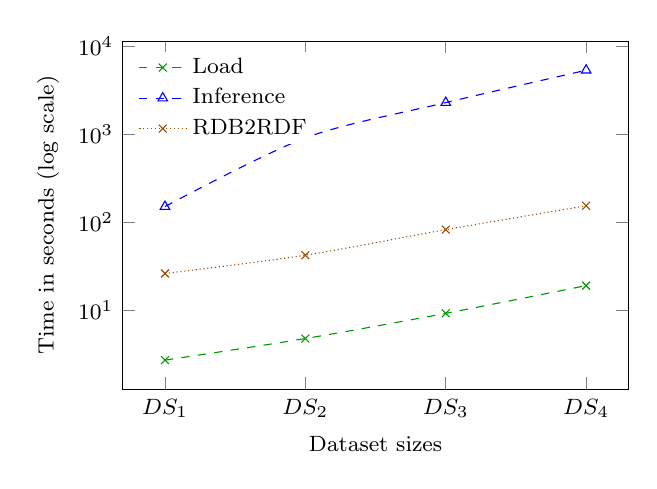
\begin{tikzpicture}
  \begin{loglogaxis}[xlabel={Dataset sizes},ylabel={Time in seconds (log scale)},%
    scaled x ticks = false, x tick label style = {/pgf/number format/fixed},scaled y ticks = false,%
    y tick label style = {/pgf/number format/fixed},enlargelimits=true,xtick={1,2,4,8},%
    xticklabels={$DS_{1}$,$DS_{2}$,$DS_{3}$,$DS_{4}$},log basis x=10,log basis y=10,unbounded coords=jump,xminorticks=false,%
    yminorticks=false,height=6cm,width=8cm,filter discard warning=false,%
    legend style={inner sep=0,legend columns=1,draw=none,font=\tiny,at={(0,0)},anchor=south east,legend pos=north west,anchor=north west,legend cell align=left}]
\addplot[smooth,dashed, color=green!60!black, every mark/.append style={solid},mark=x,] coordinates {
(1, 2.69)
(2, 4.74)
(4, 9.17)
(8, 18.94)
};
\addlegendentry{Load}
\addplot[smooth,dashed, color=blue, every mark/.append style={solid},mark=triangle,] coordinates {
(1, 150)
(2, 906)
(4, 2281)
(8, 5322)
};
\addlegendentry{Inference}
\addplot[smooth,densely dotted, color=orange!60!black, every mark/.append style={solid},mark=x,] coordinates {
(1, 26)
(2, 42)
(4, 82)
(8, 153)
};
\addlegendentry{RDB2RDF}
\end{loglogaxis}\end{tikzpicture}

%%% Local Variables:
%%% mode: latex
%%% mode: flyspell
%%% mode: reftex
%%% TeX-master: "../../thesis"
%%% End:

    \label{fig:load-times}
  }
  \subfloat[Query execution times]{
    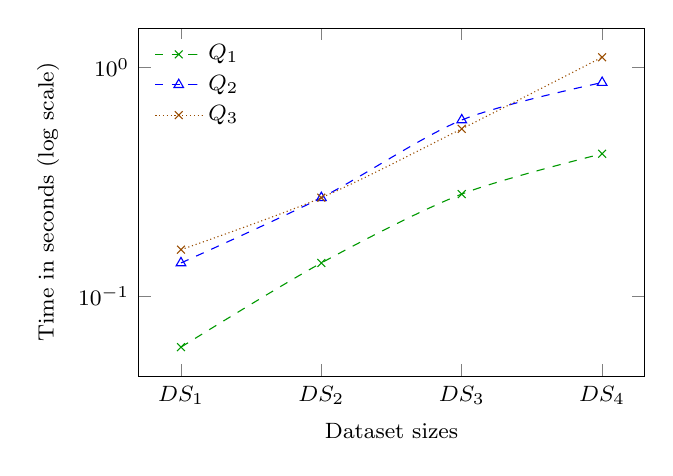
\begin{tikzpicture}
  \begin{loglogaxis}[xlabel={Dataset sizes},ylabel={Time in seconds (log scale)},%
    scaled x ticks = false, x tick label style = {/pgf/number format/fixed},scaled y ticks = false,%
    y tick label style = {/pgf/number format/fixed},enlargelimits=true,xtick={1,2,4,8},%
    xticklabels={$DS_{1}$,$DS_{2}$,$DS_{3}$,$DS_{4}$},log basis x=10,log basis y=10,unbounded coords=jump,xminorticks=false,%
    yminorticks=false,height=6cm,width=8cm,filter discard warning=false,%
    legend style={inner sep=0,legend columns=1,draw=none,font=\tiny,at={(0,0)},anchor=south east,legend pos=north west,anchor=north west,legend cell align=left}]

\addplot[smooth,dashed, color=green!60!black, every mark/.append style={solid},mark=x,] coordinates {
(1, 0.06)
(2, 0.14)
(4, 0.28)
(8, 0.42)
};
\addlegendentry{$Q_{1}$}
\addplot[smooth,dashed, color=blue, every mark/.append style={solid},mark=triangle,] coordinates {
(1, 0.14)
(2, 0.27)
(4, 0.59)
(8, 0.86)
};
\addlegendentry{$Q_{2}$}
\addplot[smooth,densely dotted, color=orange!60!black, every mark/.append style={solid},mark=x,] coordinates {
(1, 0.16)
(2, 0.27)
(4, 0.54)
(8, 1.11)
};
\addlegendentry{$Q_{3}$}
\end{loglogaxis}
\end{tikzpicture}


%%% Local Variables:
%%% mode: latex
%%% mode: flyspell
%%% mode: reftex
%%% TeX-master: "../../thesis"
%%% End:

    \label{fig:query-times}
  }
  \caption{Load and query execution times for the different Access Control datasets}
  \label{fig:load-query-times} 
\end{figure*}


%%% Local Variables:
%%% mode: latex
%%% mode: flyspell
%%% mode: reftex
%%% TeX-master: "../thesis"
%%% End:



\section{Related Work}
\label{sec:related-work}

\begin{comment}
  The use of partially ordered sets for access control has previously been considered in the domain of information flow
  in computer systems, mostly in response to the introduction of multi-user systems~\cite{Denning:1976aa}.  Although
  focusing on the question of information passing between arbitrary objects of a computer system (e.g.\ programs,
  processes or files), each process also includes a \emph{clearance class} that limits the security classes the process
  can read and write.
\end{comment}


The topic of access control has been long studied in relational databases and the approach of enforcing the access
policies by query rewriting was also considered for the Quel query language by~\citet{StonebrakerWong:1974aa}.  However,
the presented system does not rely on annotating the relational data but rather access control is specified using
constraints over the user credentials, which are then included in the rewritten query.
%
An overview of common issues, existing models and languages for access control is provided
by~\citet{VimercatiSamaratiJajodia:2005aa}.  


For the Semantic Web, well known policy languages such as KAoS~\cite{Bradshaw1997}, Rei~\cite{Kagal2003} and
PROTUNE~\cite{Bonatti2009}.  Although such languages enable policy specification using \ac{RDF} and \ac{OWL}, in their
current form they do not support reasoning based on \ac{RDF} data.  These policy languages are complimentary to our work
as they can be mapped to our annotations using rules.


\citet{DietzoldAuer2006aa} describe the requirements an \ac{RDF} store needs from a Semantic Wiki perspective.  Apart
from the necessary requirements on efficiency and scalability, the authors refer the need for access control on a triple
level and the need to integrate the structure of the organisation in the access control methods.  The described system
relies on a query engine (SPARQL is mentioned but no details are given) and a rule processor to decide the access
control enforcement at query time.
%
The system we propose in this chapter caters for both of these requirements and also integrates the access control into
the annotation query language.

\citet{HollenbachPresbreyBerners-Lee:2005aa} present the possibility of maintaing metadata on the \ac{RDF} data to
enforce access control and discuss, as possible extensions of their model, some of the work presented here, \eg~using
rules for specifying access control.  Providing access control on a resource level is also left as an open question, one
we are tackling by the specification of rules.  The extension of SPARQL is not considered.


Similar access control annotations are considered attached to axioms in an ontology
by~\citet{KnechtelStuckenschmidt:2010aa} and~\citet{BaaderKnechtelPenaloza:2009aa} and are used to allow access to
subsets of the ontology to specific users and also apply such annotations to the problem of determining the minimal set
of axioms that are necessary to support a certain conclusion.  Although the setting is different to the one presented in
this chapter, some of the algorithms for efficient annotation calculation may be ported to our modelling.


Some work on extending query languages was presented by~\citet{AbelCoiHenze2007aa}, however this work pre-dates the
SPARQL query language.  In a similar fashion to the work proposed in this chapter, their policy enforcement is also done
by a query rewriting step, however their query rewriting does not consists of including the user credentials but rather
replicating the access policies within the query.  
%
They also consider access control policies that both grant and restrict access to data.

                 
\section{Conclusion}

In this chapter we proposed an Access Control model, which can be used to protect \ac{RDF} data and demonstrate how a
combination of Annotated RDFS and SPARQL can be used to control access to integrated enterprise data.
%
This model is based on the Annotated RDFS framework presented in \cref{cha:anql} and attaches the access control
information on a triple basis, \ie~each \ac{RDF} triple can contain different annotation values.  
%
This solution provides a flexible representation method for the access control annotations, based on propositional
formul\ae{} to define which entities have access to the triple.
%
However, when considering large number of triples, challenges arise with respect to optimal access control policy
administration.  To tackle this issue we propose permission management through specifying domain-specific inference
rules for the annotation domain.
%
We also suggest a possible implementation structure for a framework to enforce the access control based on rewriting a
SPARQL query into an AnQL query.





%%% Local Variables:
%%% mode: latex
%%% mode: flyspell
%%% mode: reftex
%%% TeX-master: "../thesis"
%%% End:
